\chapter{Implementierung}

Im folgenden Kapitel wird nun auf die im Rahmen dieser Arbeit entwickelte Software eingegangen. Dazu werden zuerst allgemeine Entscheidungen erläutert, die vor der Implementation getroffen wurden. Danach wird die Implementation beschrieben, wobei einige wichtige Details näher betrachtet werden sollen. Anschließend werden anhand eines Beispiels einige Hinweise gegeben, was bei der Erweiterung der Software um weitere Protokolle zu beachten ist.

\section{Architekturentscheidungen}

\begin{mdframed}
Zugrundeliegend: Gemeinsamkeit von Protokollen, Erweiterbarkeit/Pluginfähigkeit, ...

Warum Java? (UHH als Einstieg-> für alle verständlich und auch erweiterbar, ...)

Welche TLS-Version? Oder SSL 2.0? Aus welchen Gründen? (1.2, aktuell, demonstriert Funktionsweise und Verhinderung von Angriffen; zum \inquotes{Durchklicken} von Angriffen wäre SSL schöner, ...)

Welche Dinge werden betrachtet, welche ausgelassen (Extensions, Zertifikatvalidierung, ...), aus welchen Gründen?

Ausgelassen:
\begin{itemize}
\item TLS-Extensions
\item Zertifikatsvalidierung, PKI und Verwandtes
\item Komprimierung
\item eingeschränkte Anzahl von CipherSuites (und Schlüsselaustausch)
\item Ältere Versionen
\item Clientauthentifizierung
\item Fragmentierung oder mehrere TlsMessages in einem Record
\item sichere Schlüsselverwaltung, RSA-Bleichenbacher (Noch implementieren?) 
\end{itemize}

Analyse (Rückgriff auf Didaktik-Kapitel)
\end{mdframed}

Die Wahl der Programmiersprache fiel auf Java, da diese Sprache an der Universität Hamburg in der ersten Semestern zum Einsatz kommt und von den Studierenden zwingend gelernt werden muss. Auf diese Weise sollte die entwickelte Software auch von anderen Studierenden erweitert oder zumindest problemlos verstanden werden können. Zur Erzeugung der Benutzeroberfläche wurde die in der Java-Runtime verfügbare Bibliothek Swing genutzt, da diese ebenfalls in den an der Universität Hamburg verwendet wird.

Für diese Arbeit wurde die TLS 1.2-Spezifikation umgesetzt. Hierdurch lässt sich die zum jetzigen Zeitpunkt aktuelle Version explorieren und insbesondere Abwehrmechanismen gegen Angriffe auf ältere Protokollversionen erkennen. Um diese Angriffe beobachten zu können, hätte sich auch eine ältere Protokollversion wie SSL 2.0 angeboten. Durch die Erweiterbarkeit der Software wäre dieses eine Möglichkeit für spätere Arbeiten.

Einige Funktionen der Spezifikation wurden nicht implementiert. Dies geschah aus Gründen der Komplexitätsreduktion zum besseren Verständnis oder schlicht aus Zeitgründen, insbesondere wenn die Funktion wenig zum Verständnis beigetragen hätte. Im Folgenden soll kurz auf diese Funktionen und darauf, warum sie ausgelassen wurden, eingegangen werden.\\
Auf TLS-Extensions wurde komplett verzichtet, da sie nicht für das grundsätzliche Verständnis von TLS notwendig sind, sondern eher technische Erweiterungen des Standards darstellen, um bestimmte Funktionen nachzurüsten oder Verhalten zu erzwingen.\\
Auch die Möglichkeit TLS-Plaintexte vor dem Verschlüsseln zu komprimieren wurde nicht implementiert, da die Funktion wenig zum Verständnis beiträgt und zusätzlich aufgrund ihrer Angreifbarkeit in der nächsten Protokollversion nicht mehr enthalten sein wird (vgl. Abschnitt \ref{sec_attack_crime}).\\
TLS unterstützt optional zusätzliche Clientauthentifizierung. Diese wird allerdings in vielen Anwendungsfällen, wie beim dem verschlüsselten Abruf einer Internetseite über HTTPS, nicht genutzt und unterscheidet sich prinzipiell nicht übermäßig von der Serverauthentifizierung. Daher wurde in der Software darauf verzichtet.\\
Weiterhin wurden nur einige \ciphersuites implementiert. Hierbei wurde jedoch darauf geachtet, dass sowohl Block- und AEAD-Chiffren zur Ver- und Entschlüsselung als auch RSA und das Diffie-Hellman-Verfahren zum Schlüsselaustausch verwendet wurden. Auf die Implementierung von \ciphersuites, die sich lediglich in Schlüssellängen von bereits implementierten \ciphersuites unterschieden oder deren Chiffren bzw. Schlüsselaustauschalgorithmen bereits durch andere \ciphersuites abgedeckt waren, wurde bewusst verzichtet.\\
Auch die sichere Verwaltung von Schlüsseln im Dateisystem, sowie die Entfernung verwendeter Schlüssel aus dem Speicher, auf die in produktiv verwendeten Systemen geachtet werden muss, wurde hier aus naheliegenden Gründen vernachlässigt.\\
\todo{Abbreviated Handshake? Wahrscheinlich schon!}
Ein letzter Punkt, der in der Software nicht implementiert wurde, ist die Zertifikatsvalidierung. Diese ist zwar entscheidend für den sicheren Aufbau einer Verbindung, hat aber eher indirekt mit der der Protokollspezifikation zu tun. Daher wurde aus Zeitgründen auf diese Funktion verzichtet, die sich jedoch für spätere Arbeiten anbieten würde.

\section{Implementation notes}

\begin{mdframed}
Entwurf (UML ist toll, Automatenmodelle, ...), Implementierung, Tests, Evaluation...

Probleme/Schwierigkeiten bei der Umsetzung, ...

- Abstrakt \& Architektur: Automaten und States, ViewProvider, ...\\
- TLS: PDU-Struktur (insbesondere Fragment und CipherArten), Automaten (Security Parameters, Current/Pending States, ...), States (allgemein immer für Warten auf oder Received...), Crypto, Package-Struktur
\end{mdframed}

\begin{figure}[H]
	\centering
	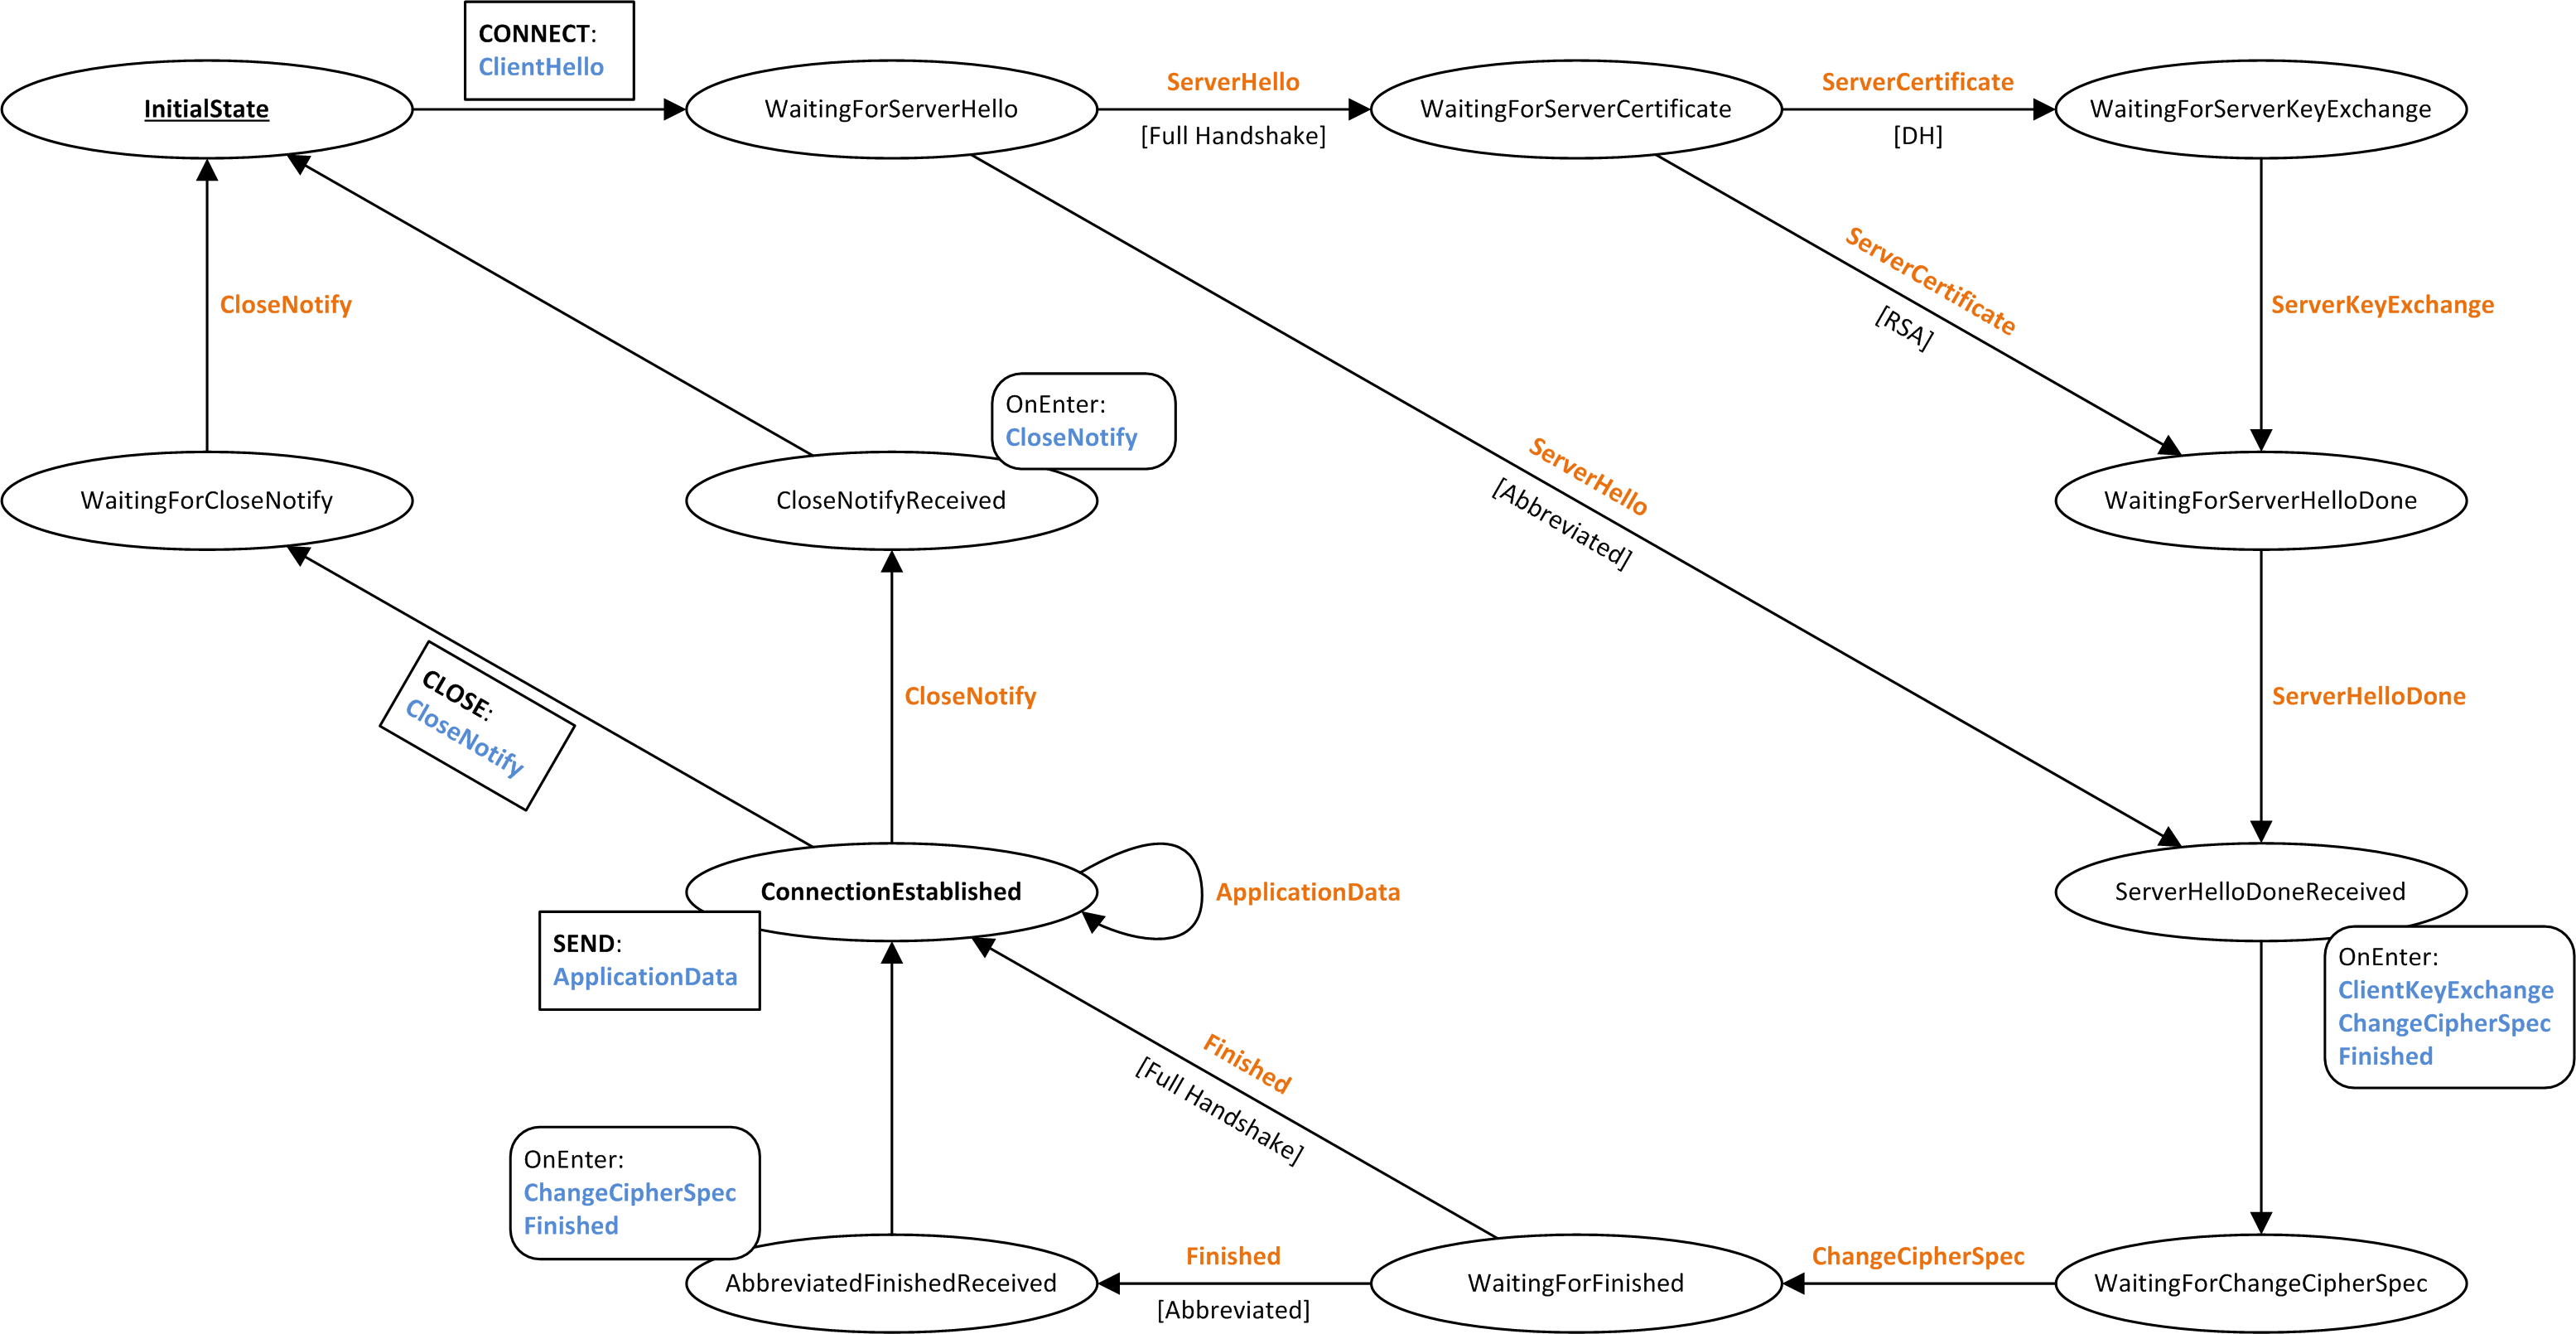
\includegraphics[scale=0.75, angle = 90]{Diagrams/client_state_machine.png} %
	\caption{Der Automat für den TLS-Client}
	\label{fig_tls_client_state_machine}
\end{figure}

\begin{figure}[H]
	\centering
	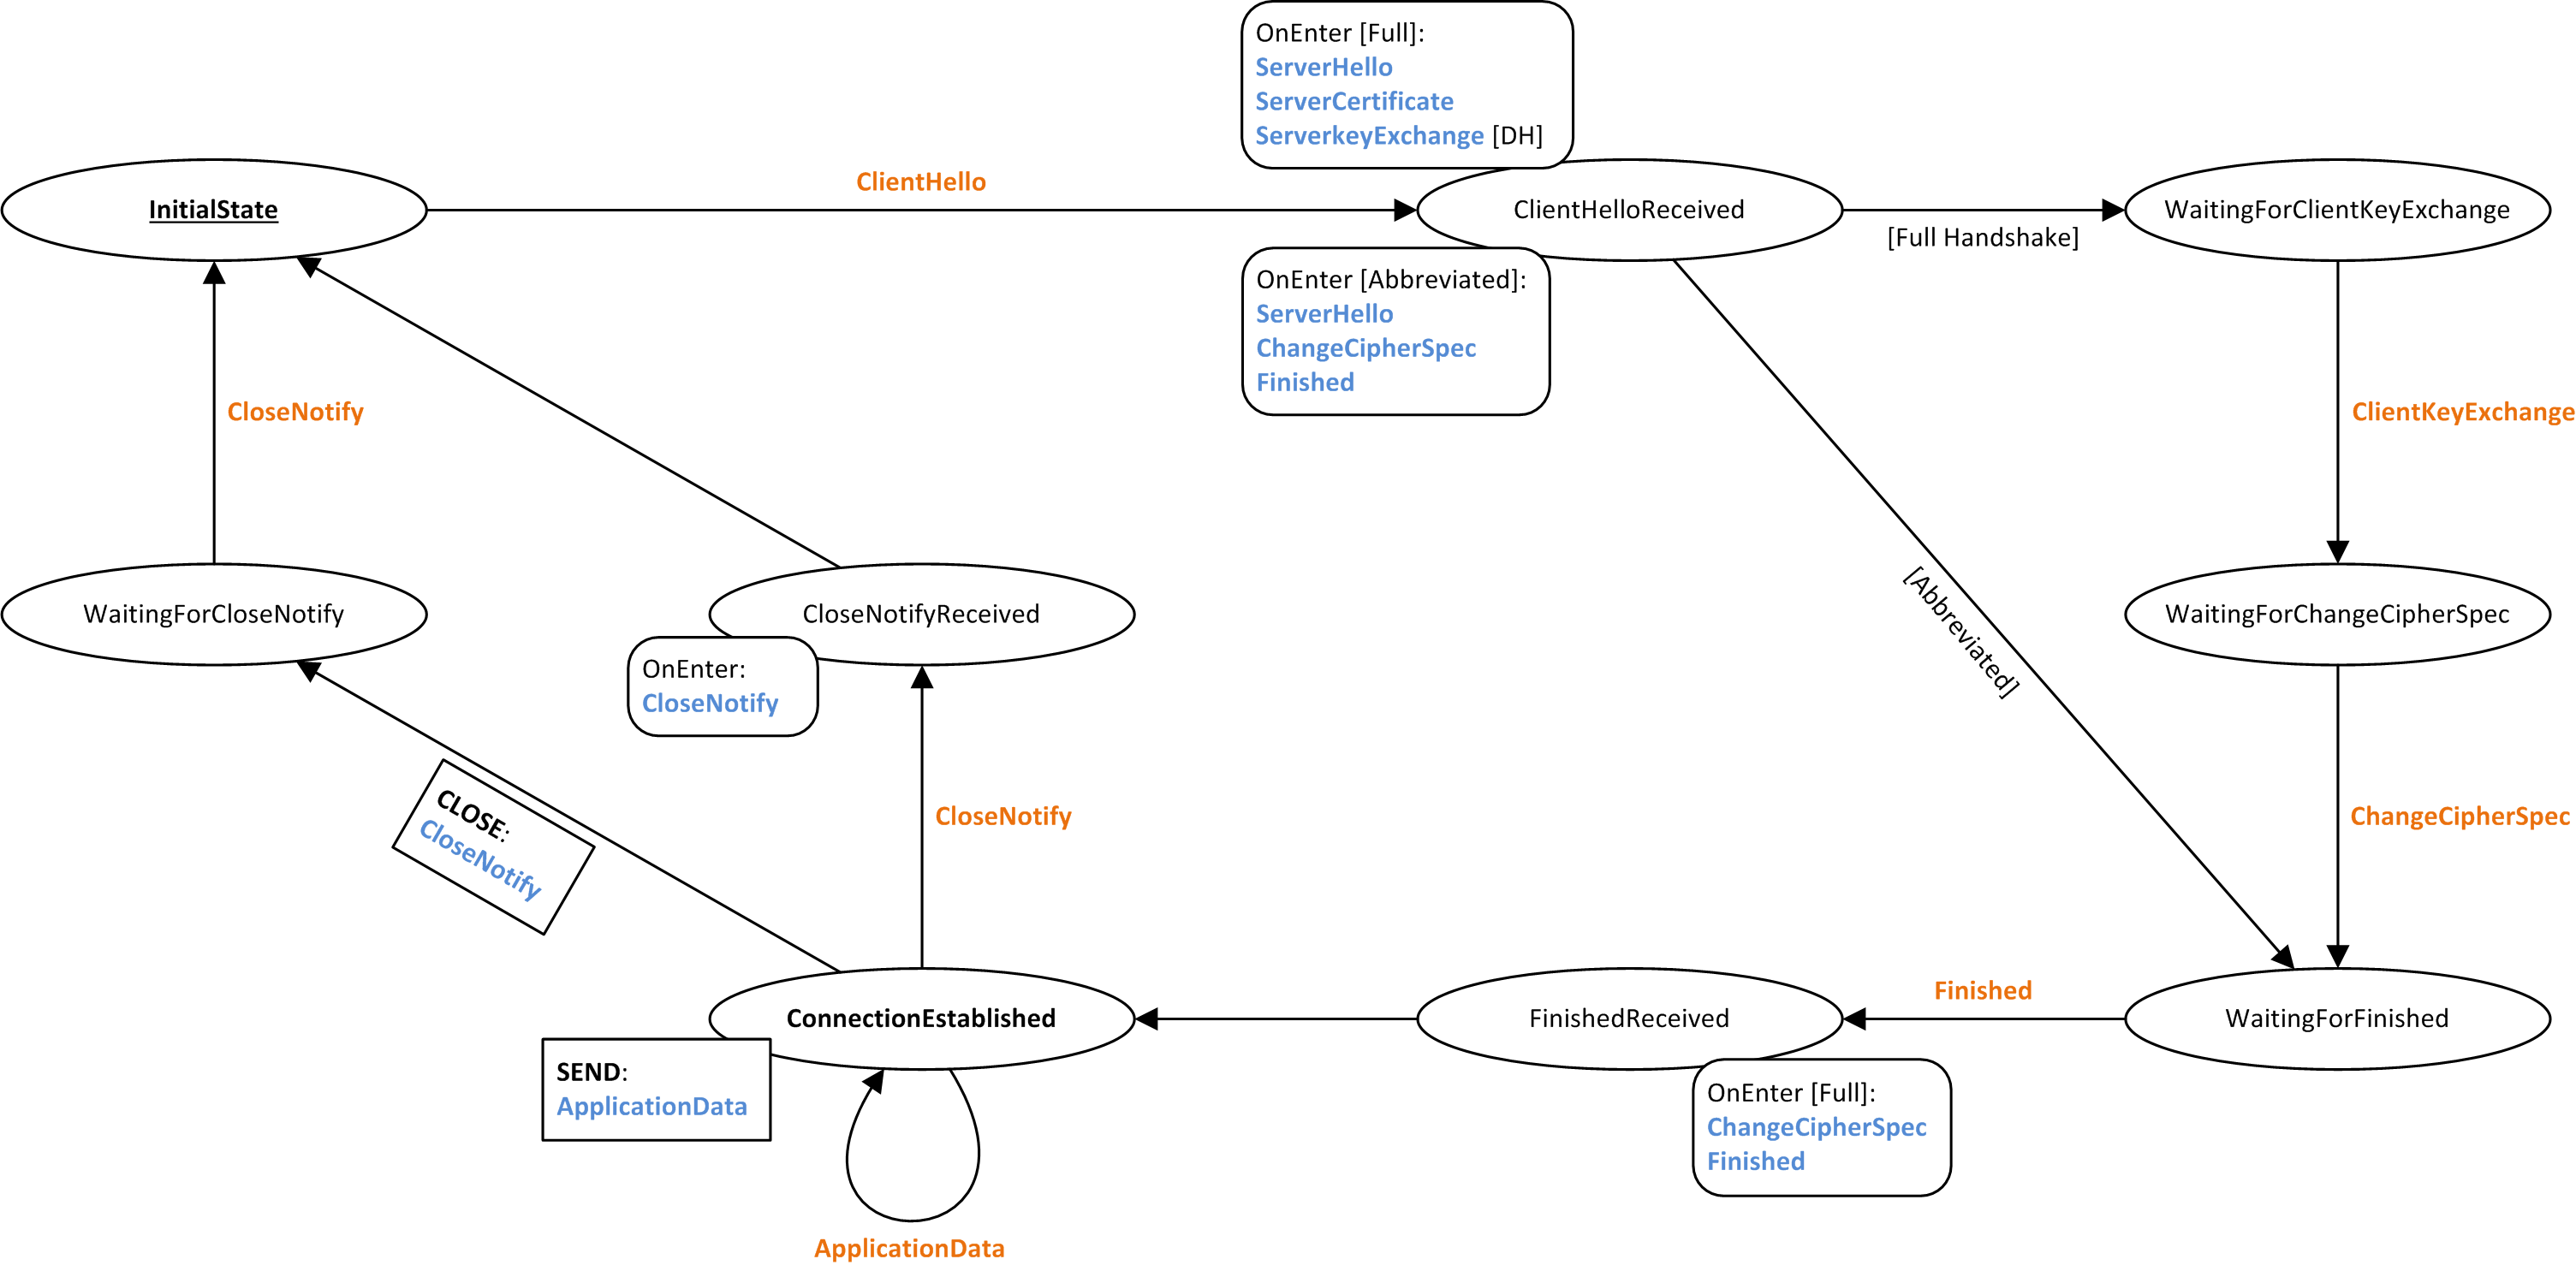
\includegraphics[scale=0.75, angle = 90]{Diagrams/server_state_machine.png} %
	\caption{Der Automat für den TLS-Server}
	\label{fig_tls_server_state_machine}
\end{figure}

\section{Tutorial: So schreibe ich ein Plugin, ...}
